\hypertarget{elektronica}{%
\section{Elektronica}\label{elektronica}}

Het programmeren was erg afhankelijk van de hardware keuzes. Als
microcontroller hebben we uiteindelijk gekozen voor de Arduino Nano.
Toen wij begonnen met ons te verdiepen in het onderwerp, raakten we
steeds meer bekend met de Raspberry Pi. Toch ontdekten we later dat dit
niet de beste microcontroller is voor een prothesehand. Omdat dit een
microcomputer is, en dus geen microcontroller, is het veel ingewikkelder
om ons project ermee uit te werken. Ook is de Raspberry Pi vrij groot.
Het voordeel aan de Raspberry Pi is wel dat je hiermee veelal Python
scripts runt. Deze taal beheersten we alledrie al vrij goed, in
tegenstelling tot C++, waar Arduino op gebaseerd is.

Er zijn veel verschillende soorten microcontrollers van Arduino. Wij
hebben hierbij voor de Nano gekozen, aangezien deze erg klein is. Toch
bezit deze controller genoeg pins\footnote{Een bepaald soort aansluiting
  bij elektronica; kleine geleidende pinnetjes.} om alles op aan te
sluiten. Ook de Arduino programmeren gaat gepaard met groot
gebruiksgemak: Je schrijft wat code op je computer, \emph{upload} deze
code naar de Arduino met de IDE en de Arduino blijft deze code
uitvoeren, in kindertaal omschreven in Vervloesem en Overman (2017).

\hypertarget{clone}{%
\subsection{Clone}\label{clone}}

Arduino is geheel open-source. Dit betekent dat alle broncode vrij op
het internet beschikbaar is. Deze vrijheid zorgt ervoor dat er vele
clones\footnote{Precies nagemaakte Arduino controllers.} van de Arduino
controllers bestaan. Dit zijn, veelal chinese, namaak Arduino's.
Hierdoor zijn er Arduino's die worden verkocht voor ongeveer één vierde
van de originele prijs. Er zijn echter niet alleen maar voordelen. De
Nano die wij hadden gekocht had een OEM driver\footnote{Een driver of
  stuurprogramma legt een verbinding tussen de hardware en het
  besturingssysteem.} voor de CH34X chipset. Dit is een andere
driver/chipset dan het origineel. Dit zorgde er helaas voor dat de
Arduino crashte in combinatie met macOS. Hierdoor komt de Arduino niet
tussen de beschikbare apparaten te staan. Dit is nodig voor het
programmeren, meer hierover in sectie 7. Na wat zoeken op het internet
kwamen wij op een repository\footnote{Een pagina op Github.com met
  open-source code.} van Mihalko (2017), waarin het probleem alsvolgt
werd omschreven: ``\emph{Version 1.3 (\ldots{}) of the OEM driver for
the CH34x chipset currently causes a kernel panic (a.k.a. crash) when
installed on macOS Sierra.}''. Hij heeft dit opgelost door een
bestandje, dat standaard zit inbegrepen bij macOS, te herschrijven.
Hierdoor werd onze clone weer herkend door Mac computers.

\hypertarget{overige-hardware}{%
\subsection{Overige hardware}\label{overige-hardware}}

Natuurlijk heb je nog veel meer hardware nodig om een hand uiteindelijk
te laten bewegen. Bijvoorbeeld de motortjes. Deze zijn grofweg in drie
categorieën in te delen: DC-motoren, stappenmotoren en servomotoren.

\begin{itemize}
\tightlist
\item
  Een DC\footnote{DC = Direct Current.} draait continu zo lang als er
  stroom op staat. Ze zijn tweedradig (power en ground) en draaien
  meestal met een hoog RPM.\footnote{RPM = Revolutions Per Minute. Het
    aantal rondjes per minuut die de motor draait.}
\end{itemize}

\begin{itemize}
\item
  Een stappenmotor werkt een stuk ingewikkelder, met meerdere
  elektromagneten die om een centraal tandwiel staan. De stappenmotor
  werkt in stapjes, en is dus erg precies te besturen. Het RPM is een
  stuk lager dan bij een DC-motor, maar de torque (draaikracht) is erg
  hoog. Een stappenmotor is echter wel vijfdradig.
\item
  Een servo is een snelle, precieze elektromotor. Meestal kan deze maar
  in 180 graden bewegen. Werkt ongeveer hetzelfde als een stappenmotor.
\end{itemize}

Het verschil tussen deze motoren wordt uitgebreider omschreven in
ModMyPi (2013).

Wij hebben uiteindelijk gekozen voor de servomotor omdat deze het best
bij een robotarm past. De motor beweegt snel, heeft maar een verbinding
naar de Arduino en heeft genoeg torque. Echter is het allerbelangrijkste
aan servomotoren dat ze feedback naar de Arduino kunnen sturen. We
kunnen dus weten in welke positie hij staat. Dit is belangrijk bij het
aansturen van de motor. Als deze bijvoorbeeld al volledig naar rechts is
gedraaid, kunnen we niet nogmaals de opdracht geven om verder naar
rechts te draaien. In ons geval zou de vinger dan door buigen. Wij zijn
uiteindelijk gekomen op de SG90. Dit is een zeer kleine, maar krachtige
servomotor. Deze motor is hieronder afgebeeld, met de bijbehorende
dimensies.

\begin{figure}
\centering
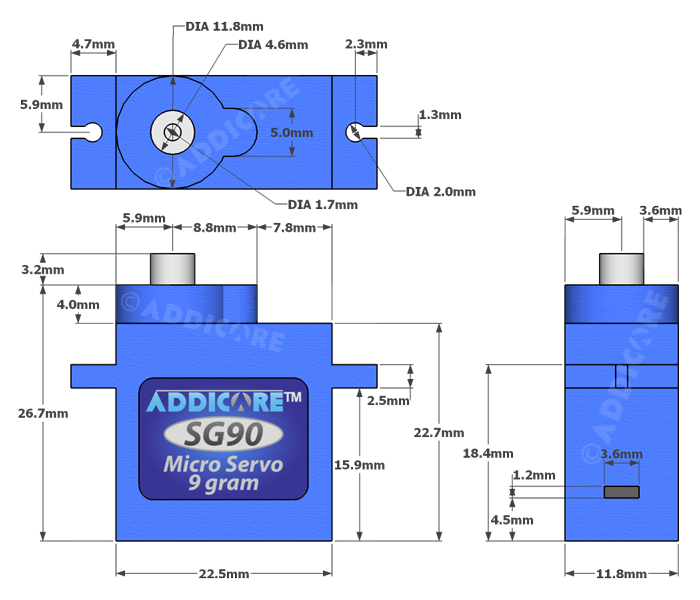
\includegraphics[width=0.4\textwidth,height=\textheight]{img/image_21.png}
\caption{De dimensies van de SG90 Mini Servo\label{fig:servo}}
\end{figure}

\hypertarget{het-aansturen-van-de-hand}{%
\subsection{Het aansturen van de hand}\label{het-aansturen-van-de-hand}}

Zoals omschreven in de theorie, is het mogelijk om de hand aan te sturen
door het kijken naar elektrische signalen in de armspieren. Dit wordt
gedaan met behulp van een EMG sensor. Een voorbeeld van een EMG sensor
is de MyoWare Muscle Sensor van Sparkfun. Deze kleine sensor is zeer
eenvoudig in gebruik en gemaakt voor microcontrollers.

Bij het plaatsen van deze sensor is het belangrijk hoe deze geplaatst
wordt. De sensoren moeten in het midden van de spier en in dezelfde
richting als de vezels zitten.

De output van de sensor is echter geen ruw EMG signaal. Het is versterkt
en de vele korte pieken zijn samengetrokken, deze specificaties staan in
de datasheet van de MyoWare: Advancer Technologies (2015). Dit verschil
is geïllustreerd in \xrefname{Fig.}\cref{fig:emg}, waar raw al versterkt
is, rectified rechtgetrokken is en integrated de samengetrokken pieken
zijn.

\begin{figure}
\centering
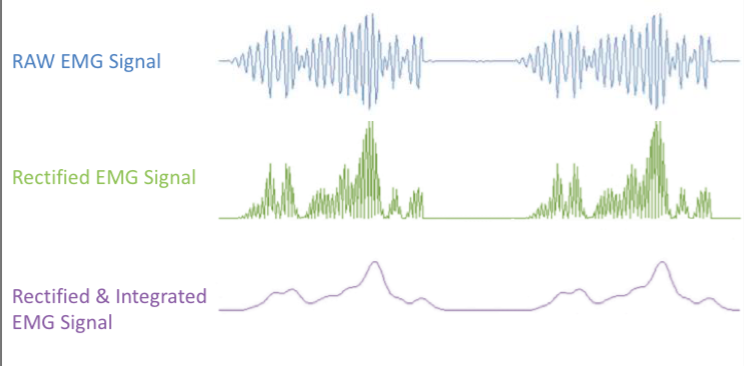
\includegraphics[width=0.54\textwidth,height=\textheight]{img/image_22.png}
\caption{Verschillende EMG signalen\label{fig:emg}}
\end{figure}

Ook de bedrading en signaalgeving werkt erg goed bij de MyoWare. Er zijn
maar drie draden voor nodig: \texttt{V+},\footnote{V+ geeft de
  stroomtoevoer weer.} \texttt{SIG}\footnote{SIG geeft de signaaldraad
  weer. Hierdoor loopt het signaal van de sensor naar de
  microcontroller.} en \texttt{GND}.\footnote{GND is de ground. Dit is
  de stroomafvoer.}

\hypertarget{elektriciteitsschema}{%
\subsection{Elektriciteitsschema}\label{elektriciteitsschema}}

Voor je begint met het werken met circuits, is het belangrijk dat de
stroomkringen altijd goed uitgedacht zijn. Als dit niet het geval is,
kan er bijvoorbeeld kortsluiting optreden. Het is hierom dan ook
belangrijk om een elektriciteitsschema van te voren te maken. Dit deden
wij met Fritzing. Fritzing is een gebruiksvriendelijke applicatie voor
het maken van zulke schema's. Fritzing ondersteunt drie verschillende
soorten weergaves: Breadboard, Schematic en PCB. Breadboard is erg
visueel. Je gebruikt hier dan ook getekende versies van echt bestaande
onderdelen. Bij de Schematic view is dit heel anders. Schematic view
geeft, zoals de naam al zegt, een schematische weergave de stroomkring.
Breadboard wordt gebruikt voor het maken van prototypes, schematische
weergave kan zowel bij prototypes als bij het uiteindelijke gesoldeerde
product gebruikt worden.

De stroomkring van onze prothesehand zag er dan als volgt uit:

\begin{figure}
\centering
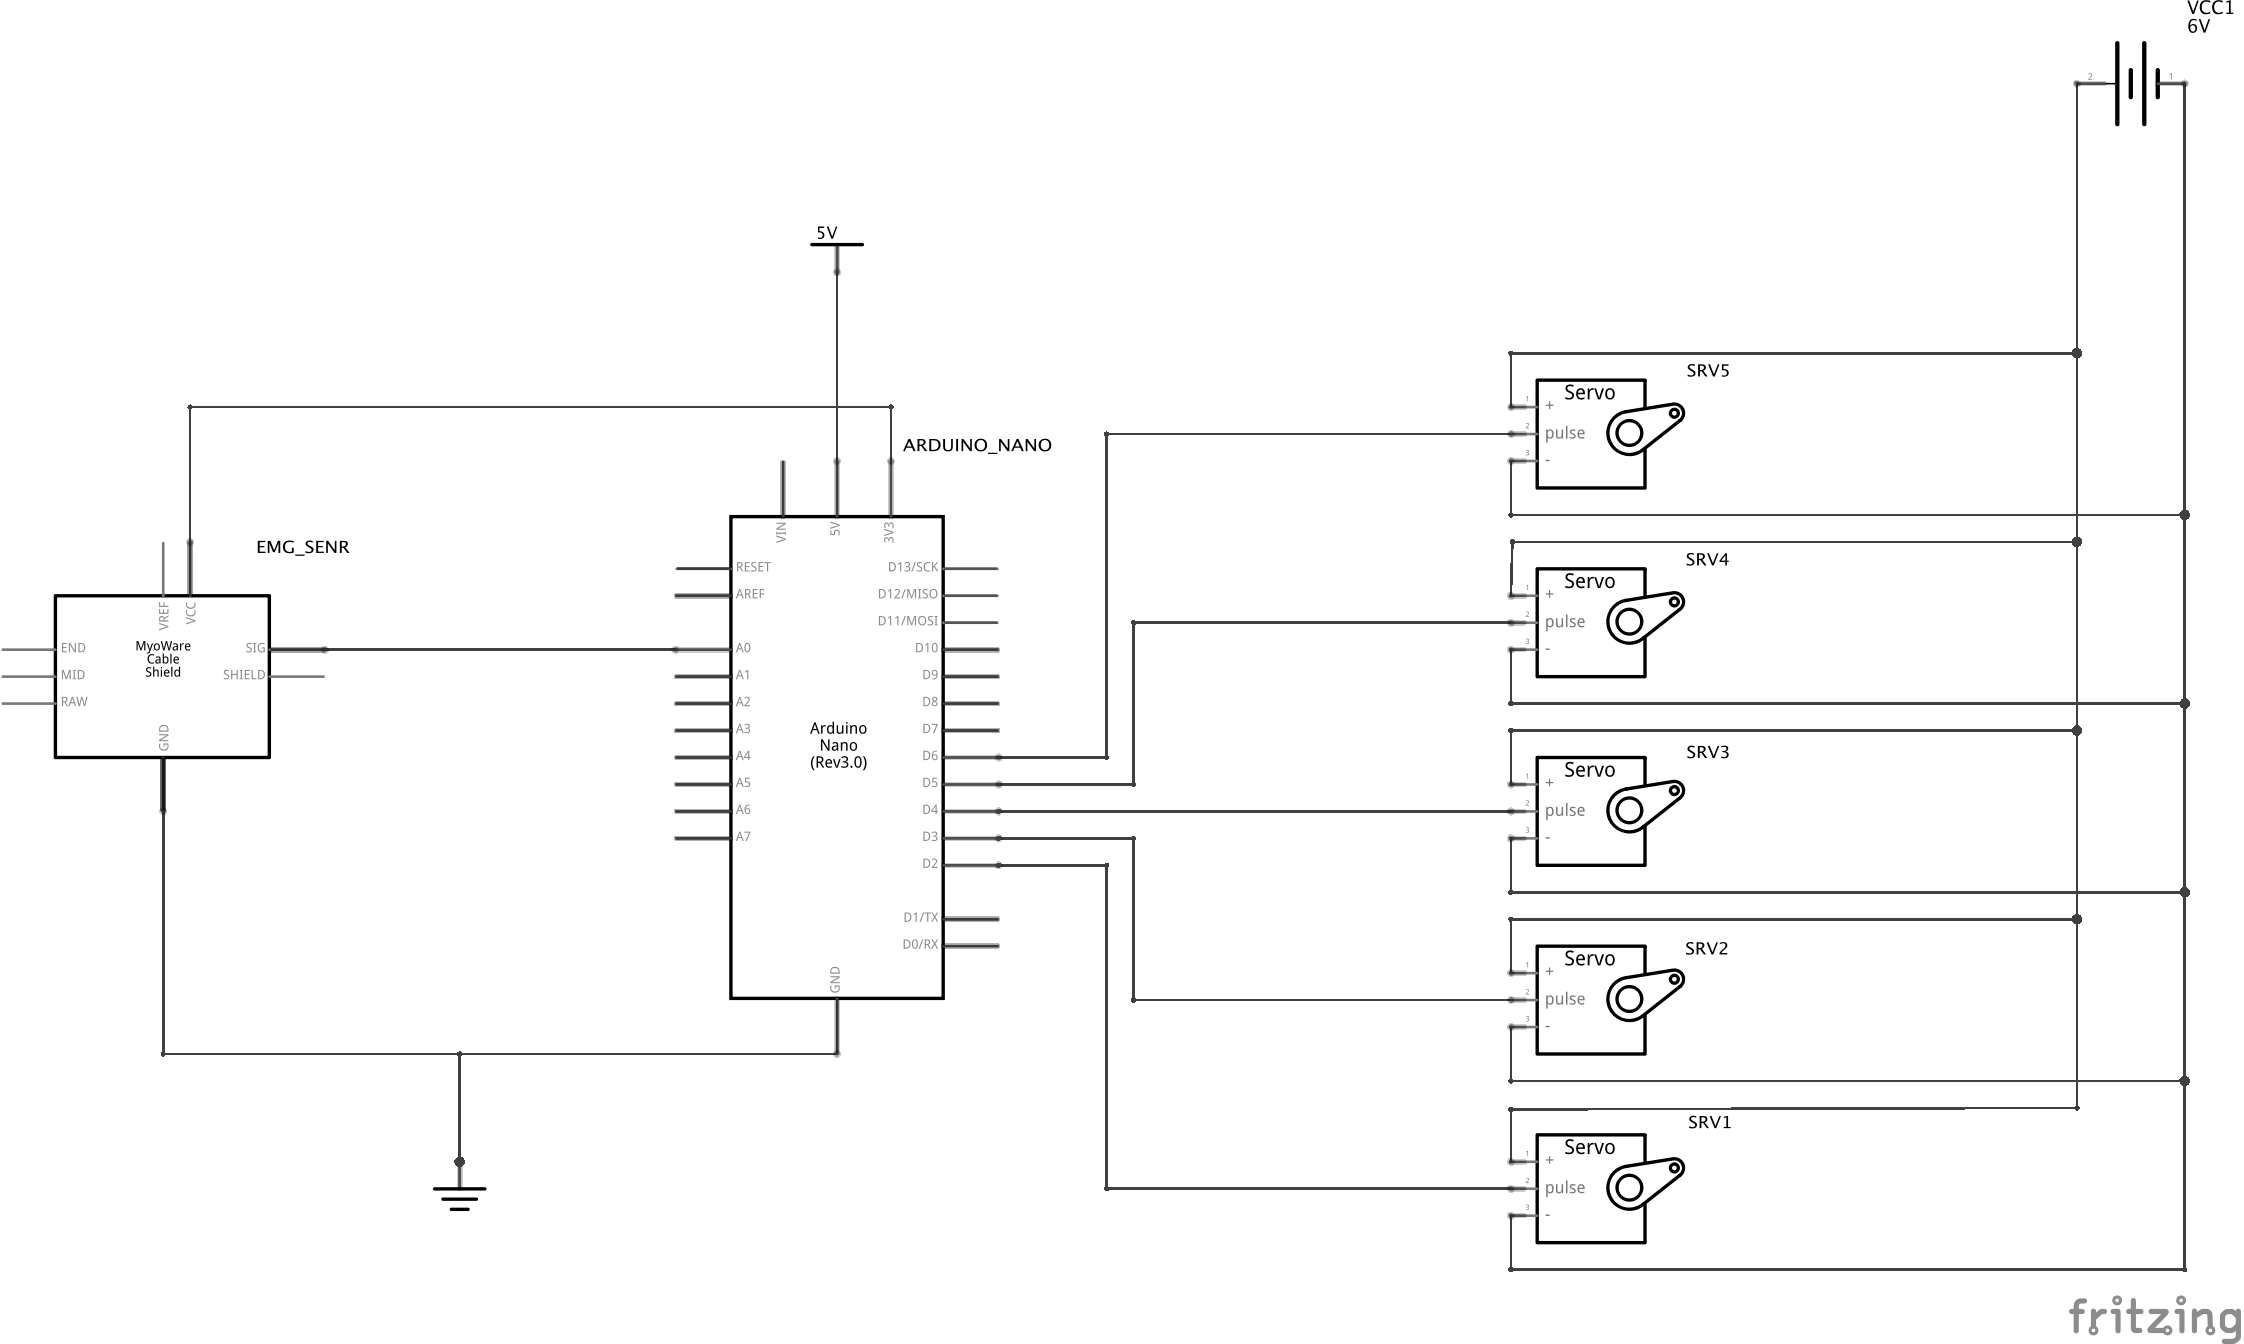
\includegraphics[width=0.65\textwidth,height=\textheight]{img/image_23.png}
\caption{Schematische weergave van stroomkring\label{fig:stroom}}
\end{figure}

Een grotere versie van dit elektriciteitsschema is te vinden in de
bijlage (\xrefname{Fig.}\cref{fig:ee}).

In het schema is te zien dat de MyoWare sensor verbonden is aan de
Arduino. Er komt stroom in vanaf de \texttt{3V3} pin van de Arduino.
Vervolgens geeft de sensor signaal af aan Arduino pin \texttt{A0}. De
Arduino en sensor hebben een gemeenschappelijke ground. Vijf digitale
pins (\texttt{D2}-\texttt{D6}) geven signaal af aan de vijf
servomotoren. Deze hebben een losse stroomkring, van 6 volt. Dit wordt
geleverd door vier in serie geschakelde AA batterijen. De 5 servomotoren
zijn aan de Arduino en bronspanning gekoppeld via een zelf ontworpen
printplaat. Dit is eigenlijk een soort driver voor de servo's.

\begin{figure}
\centering
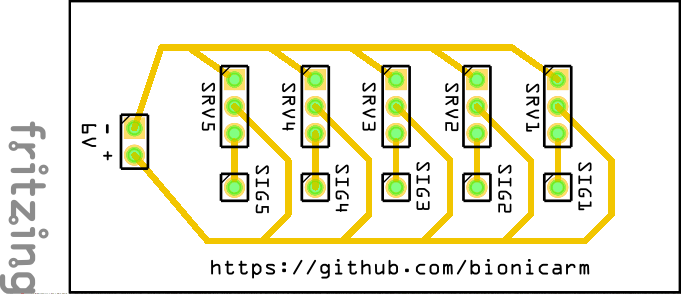
\includegraphics[width=0.58\textwidth,height=\textheight]{img/image_24_rot.png}
\caption{Servo driver printplaat. Deze is in het groot afgebeeld in de
bijlage \xrefname{Fig.}\cref{fig:driver}\label{fig:servodriver}}
\end{figure}
